\chapter{Ganeti}
\section{Introduction}


\includegraphics[width=10cm,height=7cm]{images/logo_ganeti.png}

Ganeti est un outil de gestion de machines virtuelles se basant sur les technologies de virtualisation existantes comme XEN et KVM et LXC.\\
Ganeti nécessite un logiciel de virtualisation pré-installé sur les serveurs afin de pouvoir fonctionner. Une fois installé, 
l'outil prendra en charge la partie gestion des instances virtuelles (Xen DomU), par exemple, la gestion de création de disque, 
l'installation du système d'exploitation (en coopération avec les scripts d'installation du système d'exploitation 
spécifique), et le démarrage, l'arrêt, le basculement entre les systèmes physiques. Il a été conçu pour faciliter la gestion de 
cluster de serveurs virtuels et de fournir une récupération rapide et simple.

Ganeti est un un manager de cluster de machine virtuelles. Il combine la virtualization et la réplication en temps réel de disque.
Ganeti offre un plateforme de haute disponibilité.
Ce que Ganeti peut faire d'autre :
\begin{itemize}
\item Migration en "live" des instance
\item Souplesse face aux pannes (Redondance des données avec DRBD)
\item "Cluster balancing"
\item Facilité pour les réparation et les changements matériel
\item Possibilité de superviser simultanément entre 1 et environ 200 hôtes physiques.
\end{itemize}

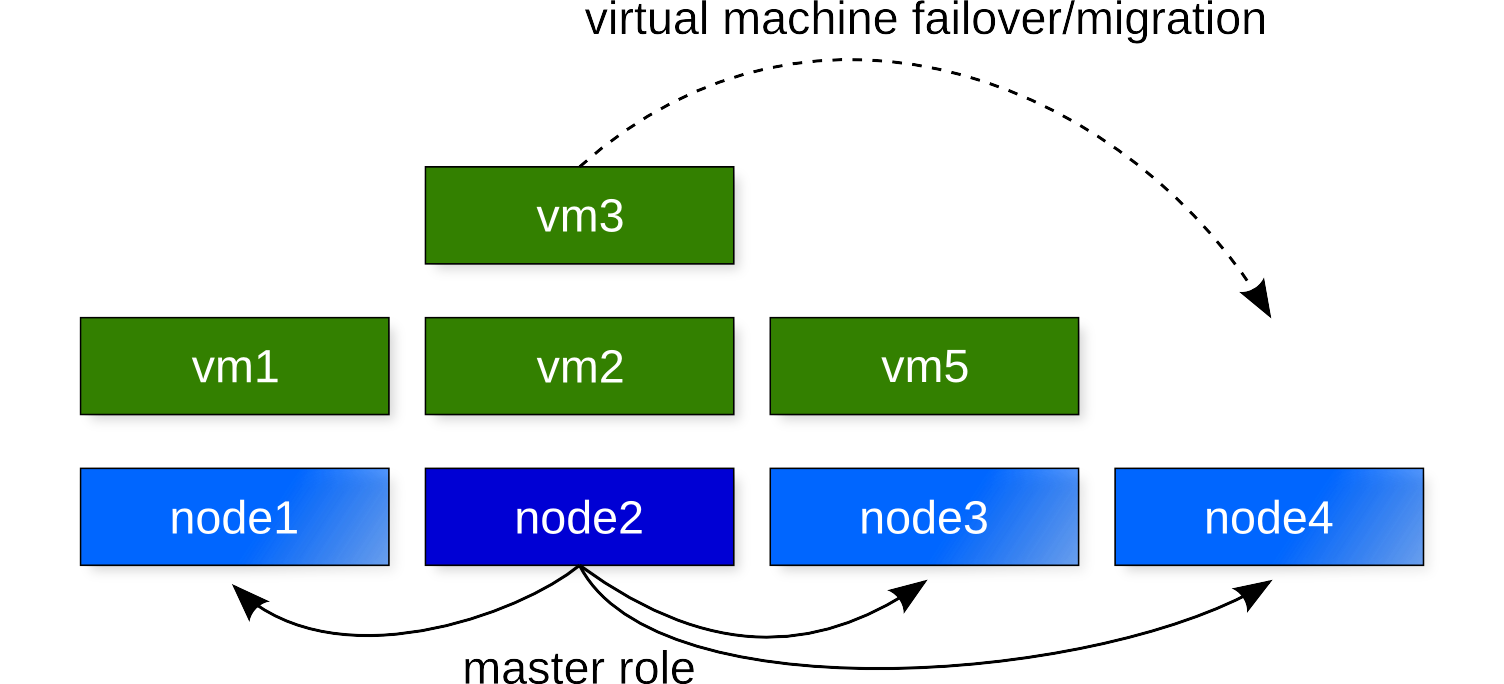
\includegraphics[width=10cm,height=7cm]{images/principe_ganeti.png}


Ganeti utilse Python, Xen, KVM, DRDB, LVM, SAN, socat et Haskell.
Développé par Google depuis Aout 2007


\includegraphics[width=10cm,height=7cm]{images/image1.png}

Ce Projet est sous licence GNU GPLv2.

Site du projet :
\begin{lstlisting}
http://code.google.com/p/ganeti/
\end{lstlisting}

Terminologie :
\begin{itemize}
\item Node : Un hôte physiques
\item Instance : Un machine virtuelles
\item Cluster : Un groupe de node supervisés
\item Job : Une opération de ganeti
\end{itemize}

\section {Installation}
\subsection {Modification des sources}
Nous avons intallé ganeti à partir de la branche testing de debian. Pour des raisons techniques le système est squeeze. Pour cela il faut ajouter les sources de testing dans le fichier /etc/apt/sources.list :
\begin{lstlisting}
##Wheezy
deb http://ftp.fr.debian.org/debian/ wheezy main contrib non-free
deb-src http://ftp.fr.debian.org/debian/ wheezy main contrib non-free

## wheezy security
deb http://security.debian.org/ wheezy/updates main contrib non-free
deb-src http://security.debian.org/ wheezy/updates main contrib non-free
\end{lstlisting}

IL faut ensuite créer le fichier de préférence de apt dans le répertoire /etc/apt/apt.conf.d. Nous avons appelé le  fichier 80default-distrib (le nom du fichier est libre). Il faut ajouter cette ligne au fichier qui défini la branche stable comme la branche par défaut :
\begin{lstlisting}
APT::Default-Release "stable";
\end{lstlisting}

\subsection {Mise à jour et installation}
On peut enfin alors mettre le système à jour et installer ganeti :

\begin{lstlisting}
apt-get update && apt-get dist-upgrade -q -y --force-yes
apt-get -t testing install -q -y --force-yes ganeti2 ganeti-htools ganeti-instance-debootstrap
\end{lstlisting}

\section {Configuration}

La configuration est l'étape la plus complexe.

\subsection {Configuration du fichier hosts}

Dans le fichier hosts il faut renseigner l'adresse et le nom complet du node primaire de cette manière :
\begin{lstlisting}
172.16.68.10    griffon-10.nancy.grid5000.fr griffon-10
\end{lstlisting}
\subsection {Copie des fichier du noyau}
Dans /etc/boot copier les fichiers vmlinuz-2.6.32-5-xen-amd64 et initrd.img-2.6.32-5-xen-amd64 :
\begin{lstlisting}
cp vmlinuz-2.6.32-5-xen-amd64 vmlinuz-2.6-xenU
cp initrd.img-2.6.32-5-xen-amd64 initrd.img-2.6-xenU
\end{lstlisting}

\subsection {Création du bridge xen-br0}

Bien que nous utilisions eth0 comme bridge, la configuration de xen-br0 dans le fichier /etc/network/interfaces est obligatoire pour l'initialisation du cluster. 

\subsection {Création du LVM}

Ganeti requière un LVM d'au moins 20Go pour fonctionner.

Sur les neud de grid5000 il est possible de créer un tel LVM sur la partition /dev/sd5.
\begin{lstlisting}
umount /dev/sda5
pvcreate /dev/sda5
vgcreate xenvg /dev/sda5
\end{lstlisting}
On a créé un VG qui se nome xenvg sur /dev/sda5.

\subsection {Edition de /usr/share/ganeti/os/debootstrap/common.sh}

Il est nécessaire d'éditer ce fichier pour que ganeti puisse créer des instances :

Par defaut le mirroir utilisé par ganeti est http://ftp.us.debian.org/debian/. Sur Grid5000 les depots US sont bloqués. Il faut donc indiquer les depots francais.
On indique aussi l'adresse du  proxy de grid5000.
On peut choisir la version de Debian que l'on souhaite installer. Ici nous avons opter pour squeeze.
L'architecture que nous choisi est amd64, car l'hote la supporte.
La variable : EXTRA\_PKGS permet d'installer des paquets supplémentaires.

\subsection {Configuration et initialisation du cluster}
L'initialisation du cluster se fait avec la commande gnt-cluster init clusterX
\begin{lstlisting}
#initialisation du cluster
gnt-cluster init --no-drbd-storage --nic-parameters link=eth0 cluster1
\end{lstlisting}
Ici nous avons précisé les options --no-drbd-storage --nic-parameters link=eth0.
La première permet d'utiliser ganeti sans utiliser la haute disponibilité.
La seconde permet de préciser un autre bridge, et d'utiliser eth0 plutôt que xen-br0

Enfin il faut renseigner le inird et le root\_path, cela est nécessaire pour la création des instances :
\begin{lstlisting}
gnt-cluster modify --hypervisor-parameter xen-pvm:initrd_path='/boot/initrd.img-2.6-xenU'
gnt-cluster modify --hypervisor-parameter xen-pvm:root_path='/dev/xvda1'
\end{lstlisting}  

\section {Utilisation des nodes}
\subsection {Ajouter un node}
Il est possible d'ajouter un node à tout moment :
\begin{lstlisting}
root@griffon-8: gnt-node add griffon-78.nancy.grid5000.fr

-- WARNING -- 
Performing this operation is going to replace the ssh daemon keypair
on the target machine (griffon-78.nancy.grid5000.fr) with the ones of the current one
and grant full intra-cluster ssh root access to/from it

Unable to verify hostkey of host griffon-78.nancy.grid5000.fr:
30:cb:8f:ec:16:6a:3b:f5:0c:2a:de:a6:4c:1d:00:19. Do you want to accept
it?
y/[n]/?: y
2012-03-12 07:38:09,239: MainThread Authentication to griffon-78.nancy.grid5000.fr via public key failed, trying password
root password:
Mon Mar 12 07:38:16 2012  - INFO: Node will be a master candidate
\end{lstlisting}
\subsection{Reconfigurer un node}
Il aussi possible de reconfigurer un node deja présent :
\begin{lstlisting}
root@griffon-8: gnt-node add --readd griffon-78.nancy.grid5000.fr

Unable to verify hostkey of host griffon-78.nancy.grid5000.fr:
6c:10:44:28:e2:2c:fc:7f:d4:5e:a3:bd:83:2c:b2:97. Do you want to accept
it?
y/[n]/?: y
Mon Mar 12 07:39:36 2012  - INFO: Readding a node, the offline/drained flags were reset
Mon Mar 12 07:39:36 2012  - INFO: Node will be a master candidate
\end{lstlisting}

\subsection {Roles des nodes et opérations}
Les différents nodes ainsi que leurs rôles :
\begin{itemize}
\item Master node : Utilise ganeti-masterd, rapi, noded and confd. Peut accueillir des instances. Toutes les opération de supervision s'effectuent sur ce node.
\item Master candidates : Possède un copie complete de la configuration, peut prendre le rôle de Master.Utilise ganeti-confd and noded. Peut accueillir des instances.
\item Regular node : Ne peuvent pas devenir Master et ne possedent qu'une partie de la configuration. Peut accueillir des instances.
\item Offline node : Ces nodes sont hors-ligne. Ne peut pas accueillir des instances.
\end{itemize}
\subsubsection {Promouvoir un neud au rang de master :}

Il faut d'abord revoquer le rang de master du node principal, sur un node master-candidate :
\begin{lstlisting}
gnt-cluster master-failover

root@griffon-81: gnt-instance list
Failure: prerequisites not met for this operation:
This is not the master node, please connect to node 'griffon-8.nancy.grid5000.fr' and rerun the command

root@griffon-81: gnt-cluster master-failover

root@griffon-81: gnt-node list
Node                         DTotal  DFree MTotal MNode MFree Pinst Sinst
griffon-8.nancy.grid5000.fr  283.2G 283.2G  16.0G  965M 14.8G     0     0
griffon-78.nancy.grid5000.fr 283.2G 283.2G  16.0G  965M 14.8G     0     0
griffon-81.nancy.grid5000.fr 283.2G 283.2G  16.0G  965M 14.8G     0     0
\end{lstlisting}
On voit que le node griffon-81 n'était pas master avant l'utilisation de la commande. Ensuite il est possible d'executer les commandes master.

\subsubsection {Passer un neud en master-candidate :}
\begin{lstlisting}
root@griffon-81: gnt-node modify -C yes griffon-8.nancy.grid5000.fr
Modified node griffon-8.nancy.grid5000.fr
 - master_candidate -> True
 - drained -> False
\end{lstlisting}
\subsubsection {Passer un node en status drained :}
\begin{lstlisting}
root@griffon-81: gnt-node modify -D yes griffon-8.nancy.grid5000.fr
Modified node griffon-8.nancy.grid5000.fr
 - master_candidate -> False
 - drained -> True
\end{lstlisting}
\subsubsection {Passer un node en offline :}
\begin{lstlisting}
root@griffon-81: gnt-node modify -O yes griffon-8.nancy.grid5000.fr
Modified node griffon-8.nancy.grid5000.fr
 - master_candidate -> False
 - offline -> True
\end{lstlisting}
\subsubsection {Passer un node en mode regular (remise à zero de tous les flags) :}
\begin{lstlisting}
root@griffon-81: gnt-node modify -O no -D no -C no griffon-8.nancy.grid5000.fr
Mon Mar 12 08:26:01 2012  - INFO: Ignoring request to unset flag master_candidate, already unset
Mon Mar 12 08:26:01 2012  - INFO: Ignoring request to unset flag drained, already unset
Mon Mar 12 08:26:01 2012  - INFO: Auto-promoting node to master candidate
Mon Mar 12 08:26:01 2012  - WARNING: Transitioning node from offline to online state without using re-add. Please make sure the node is healthy!
Modified node griffon-8.nancy.grid5000.fr
 - master_candidate -> True
 - offline -> False
\end{lstlisting}
Le node est de nouveau en master-candidate comme à l'origine.

\subsection {Supprimer un node :}
\begin{lstlisting}
root@griffon-81: gnt-node list
Node                         DTotal  DFree MTotal MNode MFree Pinst Sinst
griffon-8.nancy.grid5000.fr  283.2G 282.2G  16.0G  965M 14.7G     1     0
griffon-78.nancy.grid5000.fr 283.2G 283.2G  16.0G  965M 14.8G     0     0
griffon-81.nancy.grid5000.fr 283.2G 283.2G  16.0G  965M 14.8G     0     0

root@griffon-81: gnt-node remove griffon-78.nancy.grid5000.fr

root@griffon-81: gnt-node list
Node                         DTotal  DFree MTotal MNode MFree Pinst Sinst
griffon-8.nancy.grid5000.fr  283.2G 282.2G  16.0G  965M 14.7G     1     0
griffon-81.nancy.grid5000.fr 283.2G 283.2G  16.0G  965M 14.8G     0     0
\end{lstlisting}
Le node griffon-78 à bien été effacer du cluster.

\subsection {Manipulation du stockage :}

Faire la liste des volumes sur lesquels sont les instances : 
\begin{lstlisting}
root@griffon-81: gnt-node volumes
Node                         PhysDev   VG    Name                                        Size Instance 
griffon-81.nancy.grid5000.fr /dev/sda5 xenvg 4b328fb6-1cc9-4599-9523-2c6a8cf7b861.disk0 1000M instance4
griffon-8.nancy.grid5000.fr  /dev/sda5 xenvg 8a85c87b-39fa-4e88-886b-a60c8706cc65.disk0 1000M instance2
griffon-8.nancy.grid5000.fr  /dev/sda5 xenvg d84f3842-04d5-4951-aded-b5ea76f19681.disk0 1000M instance1
griffon-8.nancy.grid5000.fr  /dev/sda5 xenvg ddfea3fc-d7b1-4a06-ae37-3094b1f0de11.disk0 1000M instance3
\end{lstlisting}
Il est possible de lancer une reparation sur les volume de stockage :
\begin{lstlisting}
root@griffon-81:~# gnt-node repair-storage griffon-8.nancy.grid5000.fr lvm-vg xenvg
Mon Mar 12 09:56:23 2012 Repairing storage unit 'xenvg' on griffon-8.nancy.grid5000.fr ...
\end{lstlisting}
Cela équivau à vgreduce --removemissing.



\section {Utilisation des instances}

\subsection {Ajouter une instance}
\begin{lstlisting}
root@graphene-11: gnt-instance add -n graphene-11.nancy.grid5000.fr -o debootstrap+default -t plain -s 1000 instance1

Sat Mar 10 16:52:35 2012 * disk 0, vg xenvg, name 99370e22-9421-40d6-8d9d-59bb6ecfa959.disk0
Sat Mar 10 16:52:35 2012 * creating instance disks...
Sat Mar 10 16:52:36 2012 adding instance instance1 to cluster config
Sat Mar 10 16:52:36 2012  - INFO: Waiting for instance instance1 to sync disks.
Sat Mar 10 16:52:37 2012  - INFO: Instance instance1's disks are in sync.
Sat Mar 10 16:52:37 2012 * running the instance OS create scripts...
Sat Mar 10 16:54:05 2012 * starting instance...

root@graphene-11: gnt-instance list
Instance  Hypervisor OS                  Primary_node                  Status  Memory
instance1 xen-pvm    debootstrap+default graphene-11.nancy.grid5000.fr running   128M
\end{lstlisting}
L'instance est bien créer sur le neud. Il est possible à partir du maitre de créer des instances sur n'importe quels neud d'un cluster. Il aussi possible de créer une instance primaire sur un noeud et une instance secondaire sur un autre.

\subsection {Supprimer une instance}
\begin{lstlisting}
root@graphene-11: gnt-instance remove instance1
This will remove the volumes of the instance instance1 (including
mirrors), thus removing all the data of the instance. Continue?
y/[n]/?: y

root@graphene-11: gnt-instance list
Instance Hypervisor OS Primary_node Status Memory
\end{lstlisting}
L'instance à bien été supprimée. Cette commande supprime l'instance quelque soit le ou les neud où elle a été créer.


Arret et demarrage d'une instance
\begin{lstlisting}
root@graphene-11: gnt-instance list
Instance  Hypervisor OS                  Primary_node                  Status  Memory
instance1 xen-pvm    debootstrap+default graphene-11.nancy.grid5000.fr running   128M
instance2 xen-pvm    debootstrap+default graphene-11.nancy.grid5000.fr running   128M

root@graphene-11: gnt-instance shutdown instance2
Waiting for job 21 for instance2...

root@graphene-11: gnt-instance list
Instance  Hypervisor OS                  Primary_node                  Status     Memory
instance1 xen-pvm    debootstrap+default graphene-11.nancy.grid5000.fr running      128M
instance2 xen-pvm    debootstrap+default graphene-11.nancy.grid5000.fr ADMIN_down      -
\end{lstlisting}


\begin{lstlisting}
root@graphene-11: gnt-instance startup instance2
Waiting for job 26 for instance2...

root@graphene-11: gnt-instance list
Instance  Hypervisor OS                  Primary_node                  Status  Memory
instance1 xen-pvm    debootstrap+default graphene-11.nancy.grid5000.fr running   128M
instance2 xen-pvm    debootstrap+default graphene-11.nancy.grid5000.fr running   128M
\end{lstlisting}
Le status de instance2 est de nouveau "running" ce qui signifie qu'elle est en fonctionnement.

Interroger les instances :
\begin{lstlisting}
root@graphene-11: gnt-instance info instance1

Instance name: instance1
UUID: 3c3bd5ac-a261-4cba-a7f3-6cc74e49ce4e
Serial number: 2
Creation time: 2012-03-10 17:06:56
Modification time: 2012-03-10 17:07:04
State: configured to be up, actual state is up
  Nodes:
    - primary: graphene-11.nancy.grid5000.fr
    - secondaries: 
  Operating system: debootstrap+default
  Allocated network port: None
  Hypervisor: xen-pvm
    - blockdev_prefix: default (sd)
    - bootloader_args: default ()
    - bootloader_path: default ()
    - initrd_path: default (/boot/initrd.img-2.6-xenU)
    - kernel_args: default (ro)
    - kernel_path: default (/boot/vmlinuz-2.6-xenU)
    - root_path: default (/dev/sda1)
    - use_bootloader: default (False)
  Hardware:
    - VCPUs: 1
    - memory: 128MiB
    - NICs:
      - nic/0: MAC: aa:00:00:d8:c6:8a, IP: None, mode: bridged, link: xen-br0
  Disk template: plain
  Disks:
    - disk/0: lvm, size 1000M
      access mode: rw
      logical_id:  xenvg/3fe11555-edcd-40dc-bf63-f3fb749825bb.disk0
      on primary:  /dev/xenvg/3fe11555-edcd-40dc-bf63-f3fb749825bb.disk0 (254:0)
\end{lstlisting}
Cette commande édite les informations relatives à l'instance.


Import et export d'instances :

Export :
\begin{lstlisting}
root@graphene-100: gnt-backup export -n graphene-143.nancy.grid5000.fr instance1
Sun Mar 11 14:06:04 2012 Shutting down instance instance1
Sun Mar 11 14:08:07 2012 Creating a snapshot of disk/0 on node graphene-100.nancy.grid5000.fr
Sun Mar 11 14:08:08 2012 Starting instance instance1
Sun Mar 11 14:08:09 2012 Exporting snapshot/0 from graphene-100.nancy.grid5000.fr to graphene-143.nancy.grid5000.fr
Sun Mar 11 14:08:13 2012 snapshot/0 is now listening, starting export
Sun Mar 11 14:08:17 2012 snapshot/0 is receiving data on graphene-143.nancy.grid5000.fr
Sun Mar 11 14:08:17 2012 snapshot/0 is sending data on graphene-100.nancy.grid5000.fr
Sun Mar 11 14:08:22 2012 snapshot/0 sent 14M, 2.8 MiB/s
Sun Mar 11 14:08:38 2012 snapshot/0 finished receiving data
Sun Mar 11 14:08:38 2012 snapshot/0 finished sending data
Sun Mar 11 14:08:38 2012 Removing snapshot of disk/0 on node graphene-100.nancy.grid5000.fr
Sun Mar 11 14:08:39 2012 Finalizing export on graphene-143.nancy.grid5000.fr
Sun Mar 11 14:08:40 2012 Removing old exports for instance instance1
\end{lstlisting}
L'instance à bien été exporté dans graphene-143.nancy.grid5000.fr

Il est tout à fait possible d'exporter une instance sans la redémarer en utilisant l'option : --noshutdown.

Import :
\begin{lstlisting}
root@graphene-100: gnt-instance remove instance1
This will remove the volumes of the instance instance1 (including
mirrors), thus removing all the data of the instance. Continue?
y/[n]/?: y

root@graphene-100: gnt-instance list
Instance  Hypervisor OS                  Primary_node                   Status  Memory
instance2 xen-pvm    debootstrap+default graphene-100.nancy.grid5000.fr running   128M
instance3 xen-pvm    debootstrap+default graphene-143.nancy.grid5000.fr running   128M
\end{lstlisting}
Instance1 à été supprimée du cluster.
\begin{lstlisting}
root@graphene-100: gnt-backup import -n graphene-100.nancy.grid5000.fr --src-node=graphene-143.nancy.grid5000.fr -t plain instance1
Sun Mar 11 14:22:29 2012 * disk 0, vg xenvg, name a4cc7447-5ed7-4417-b222-d33a0c2842a0.disk0
Sun Mar 11 14:22:29 2012 * creating instance disks...
Sun Mar 11 14:22:30 2012 adding instance instance1 to cluster config
Sun Mar 11 14:22:30 2012  - INFO: Waiting for instance instance1 to sync disks.
Sun Mar 11 14:22:30 2012  - INFO: Instance instance1's disks are in sync.
Sun Mar 11 14:22:30 2012 * running the instance OS import scripts...
Sun Mar 11 14:22:30 2012 Exporting disk/0 from graphene-143.nancy.grid5000.fr to graphene-100.nancy.grid5000.fr
Sun Mar 11 14:22:34 2012 disk/0 is now listening, starting export
Sun Mar 11 14:22:37 2012 disk/0 is receiving data on graphene-100.nancy.grid5000.fr
Sun Mar 11 14:22:37 2012 disk/0 is sending data on graphene-143.nancy.grid5000.fr
Sun Mar 11 14:22:42 2012 disk/0 sent 34M, 6.0 MiB/s, 19%, ETA 23s
Sun Mar 11 14:23:08 2012 disk/0 finished sending data
Sun Mar 11 14:23:14 2012 disk/0 finished receiving data
\end{lstlisting}
On importe instance1 depuis graphene-143.nancy.grid5000.fr.
\begin{lstlisting}
root@graphene-100: gnt-instance list
Instance  Hypervisor OS                  Primary_node                   Status     Memory
instance1 xen-pvm    debootstrap+default graphene-100.nancy.grid5000.fr ADMIN_down      -
instance2 xen-pvm    debootstrap+default graphene-100.nancy.grid5000.fr running      128M
instance3 xen-pvm    debootstrap+default graphene-143.nancy.grid5000.fr running      128M
\end{lstlisting}
L'instance à bien été importée.
\begin{lstlisting}
root@graphene-100: gnt-instance startup instance1
Waiting for job 32 for instance1...

root@graphene-100: gnt-instance list
Instance  Hypervisor OS                  Primary_node                   Status  Memory
instance1 xen-pvm    debootstrap+default graphene-100.nancy.grid5000.fr running   128M
instance2 xen-pvm    debootstrap+default graphene-100.nancy.grid5000.fr running   128M
instance3 xen-pvm    debootstrap+default graphene-143.nancy.grid5000.fr running   128M
\end{lstlisting}
L'instance est fonctionnelle sur graphene-100.nancy.grid5000.fr

IL est aussi possible d'importer une instance étrangère à ganeti dont le disque est deja dans un LVM, sans avoir à le recopier.

\begin{lstlisting}
gnt-instance add -t plain -n HOME_NODE ... \
  --disk 0:adopt=lv_name[,vg=vg_name] INSTANCE_NAME
\end{lstlisting}

Connexion à la console d'un instance :
\begin{lstlisting}
gnt-instance console instance5
\end{lstlisting}
Une fois connecté à la console, l'utilisateur par defaut est root et il n'y pas de mots de passe.

Pour ce projet toutes nos instances sont des Debian 6.0.
Evidemment il est possible de créer des instances autres que Debian. Nous avons créer les instances à partir de debootstrap, d'autres méthodes existe.
On peut par exemple créer des instances à partir d'une image ISO. Ce qui permet d'avoir une grande variété d'instances.